\documentclass{article}
\usepackage{amsmath}
\usepackage{graphicx}

\begin{document}

\section{Numerical results for speed}

\begin{figure}[htbp]
\centering
  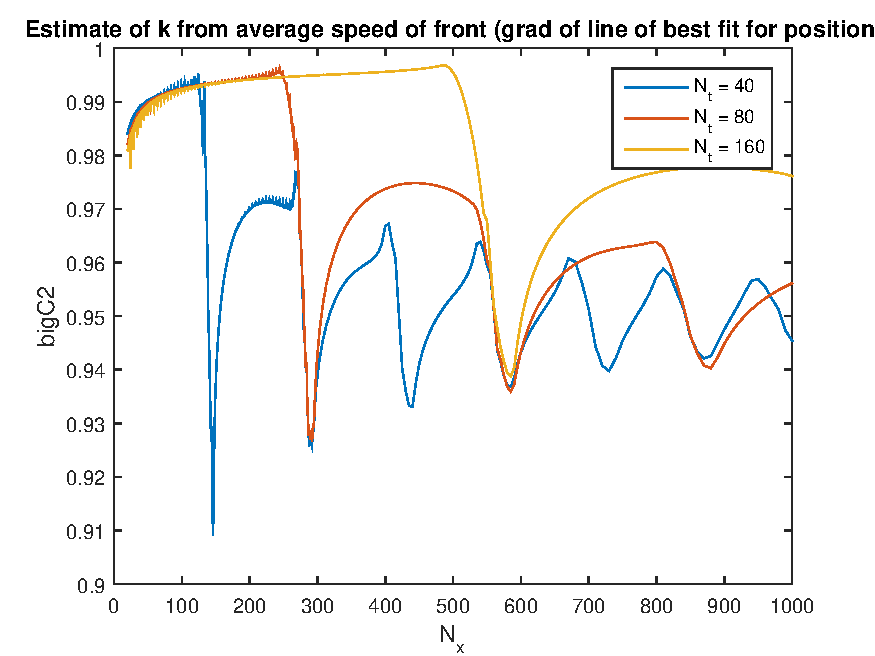
\includegraphics[width=0.9\textwidth]{alan0-k.pdf}
  \caption{Default parameters: $\alpha = 0.1$, $\theta_u = \theta_x = 0.5$,
  linear interpolation and static mesh.
  \label{fig:alan0-k}}
\end{figure}
\begin{figure}[hbtp]
\centering
  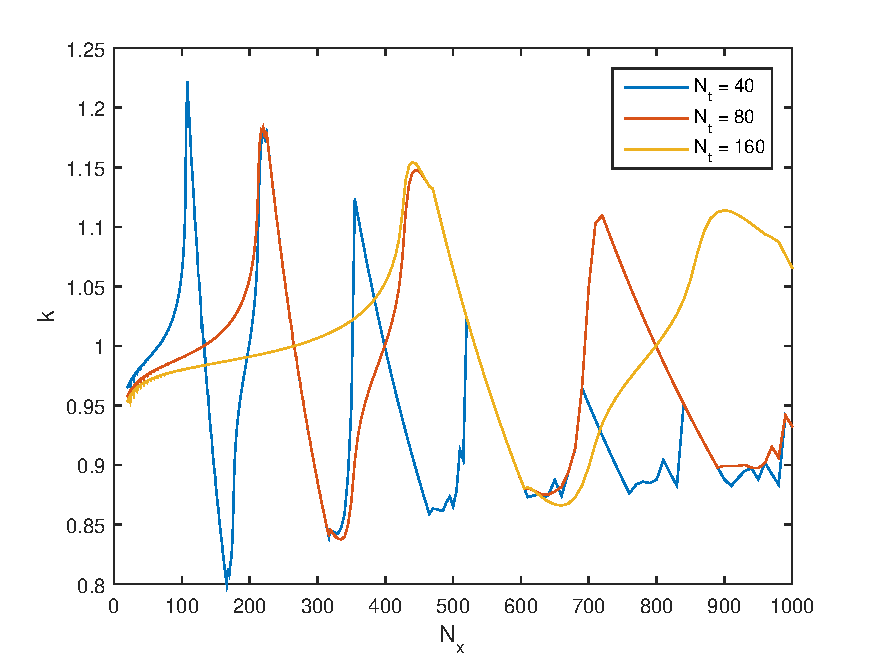
\includegraphics[width=0.9\textwidth]{alan1-k.pdf}
  \caption{As above, but $\alpha = 0.25$.
  \label{fig:alan1-k}}
\end{figure}
\begin{figure}[htbp]
\centering
  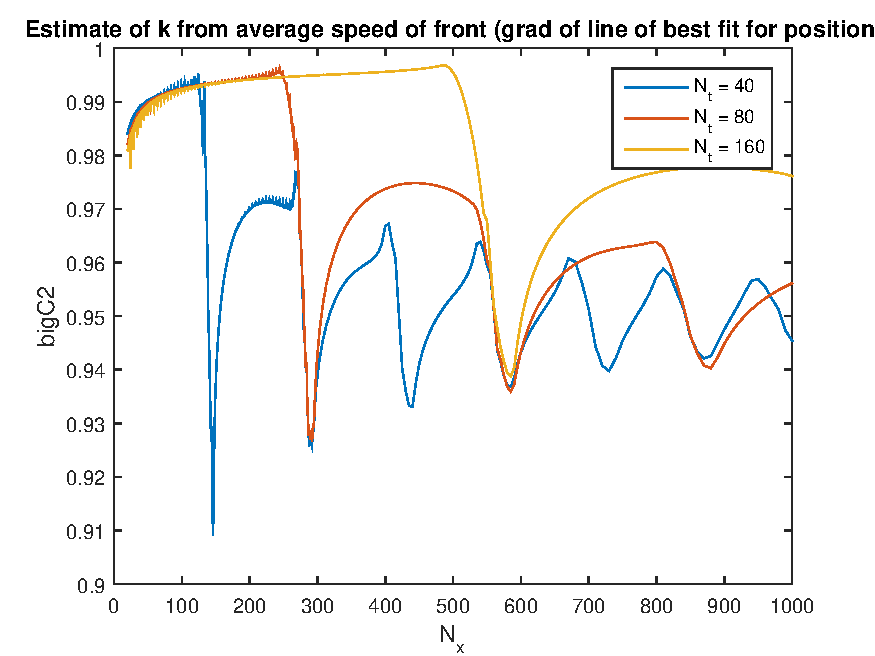
\includegraphics[width=0.9\textwidth]{alan2-k.pdf}
  \caption{Large wave amplitude, $\alpha = 0.5$.
  \label{fig:alan2-k}}
\end{figure}
\begin{figure}[hbtp]
\centering
  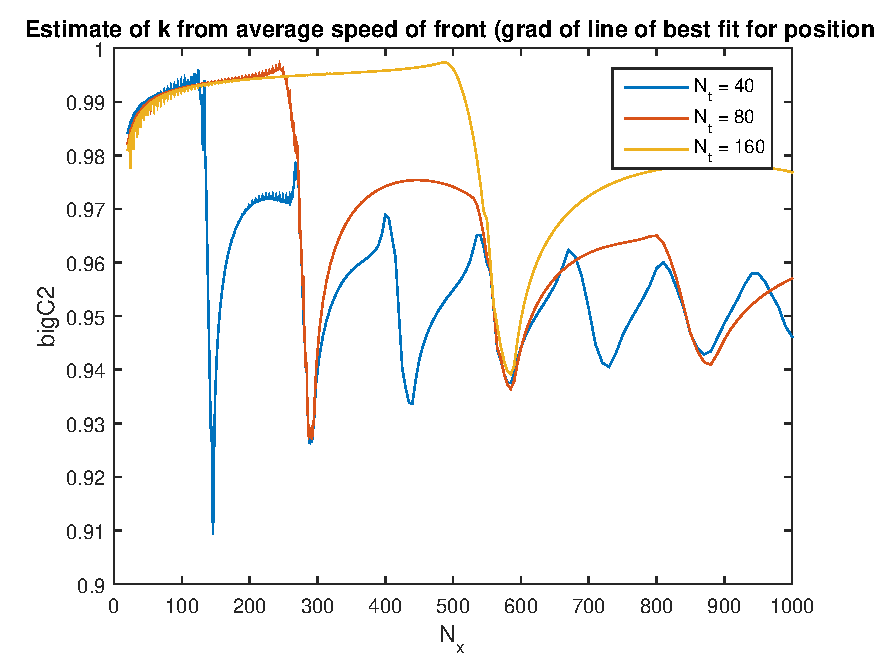
\includegraphics[width=0.9\textwidth]{alan3-k.pdf}
  \caption{Theta method in place of Crank-Nicholson with $\theta_u = \theta_x = 0.55$.
    Side-by-side, this Figure and Figure~\ref{fig:alan0-k} are indistinguishable.
  \label{fig:alan3-k}}
\end{figure}
\begin{figure}[htbp]
\centering
  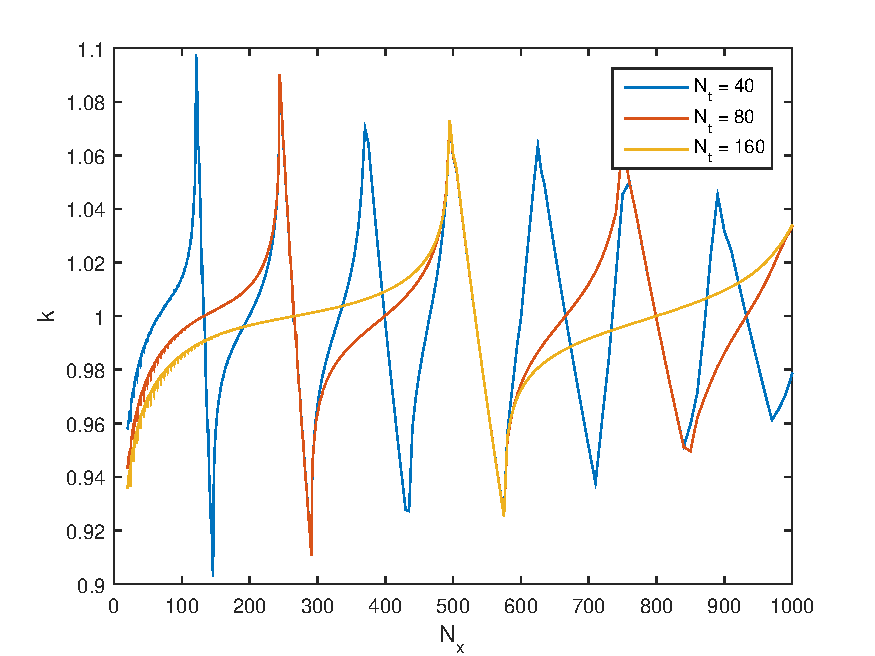
\includegraphics[width=0.9\textwidth]{alan6-k.pdf}
  \caption{Front speed using cubic Lagrange interpolation.
  \label{fig:alan6-k}}
\end{figure}
\begin{figure}[hbtp]
\centering
  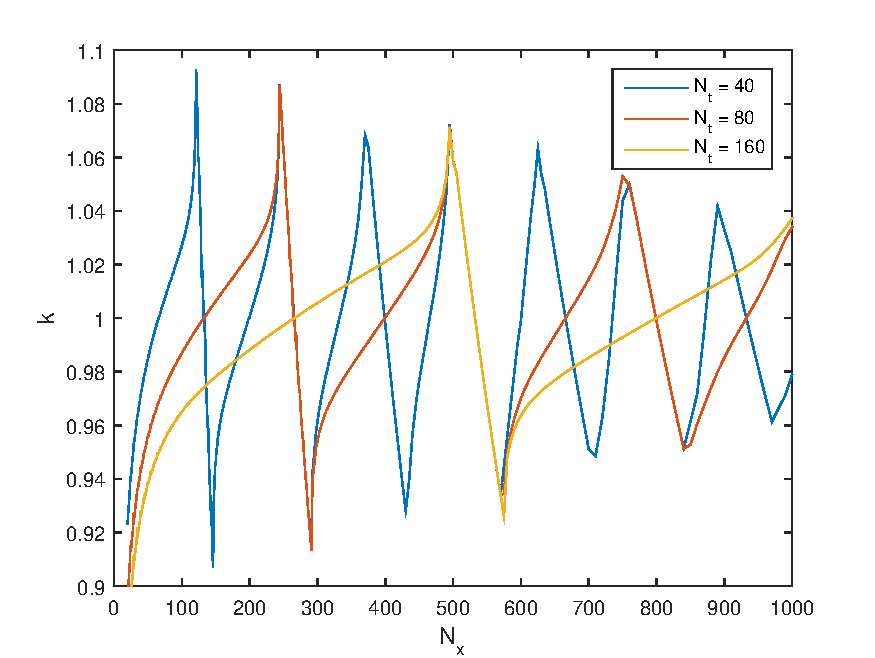
\includegraphics[width=0.9\textwidth]{alan5-k.pdf}
  \caption{As in Figure~\ref{fig:alan6-k}, but with an interpolation limiter
  applied, sacrificing smoothness for monotonicity.
  \label{fig:alan5-k}}
\end{figure}
\begin{figure}[htbp]
\centering
  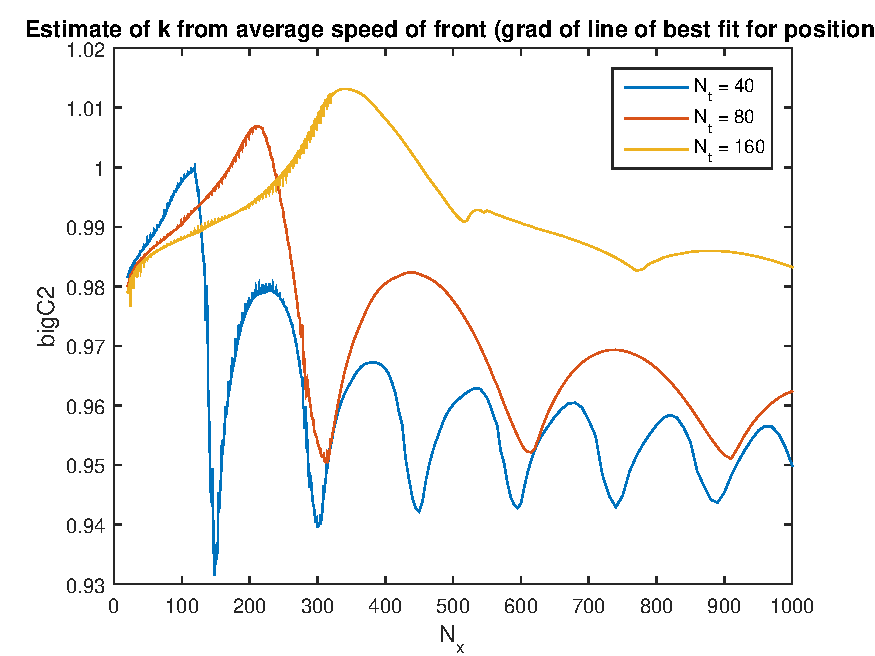
\includegraphics[width=0.9\textwidth]{alan4-k.pdf}
  \caption{Moving mesh with exact equidistribution, so $X_A^{n+1}$
    equidistributes the linear interpolant of $M(U^n_A,X^n_A)$, with
    $M(u,x) = \sqrt{0.1 + {u_x}^2}$ (after smoothing and normalisation).
  \label{fig:alan4-k}}
\end{figure}
\begin{figure}[hbtp]
\centering
  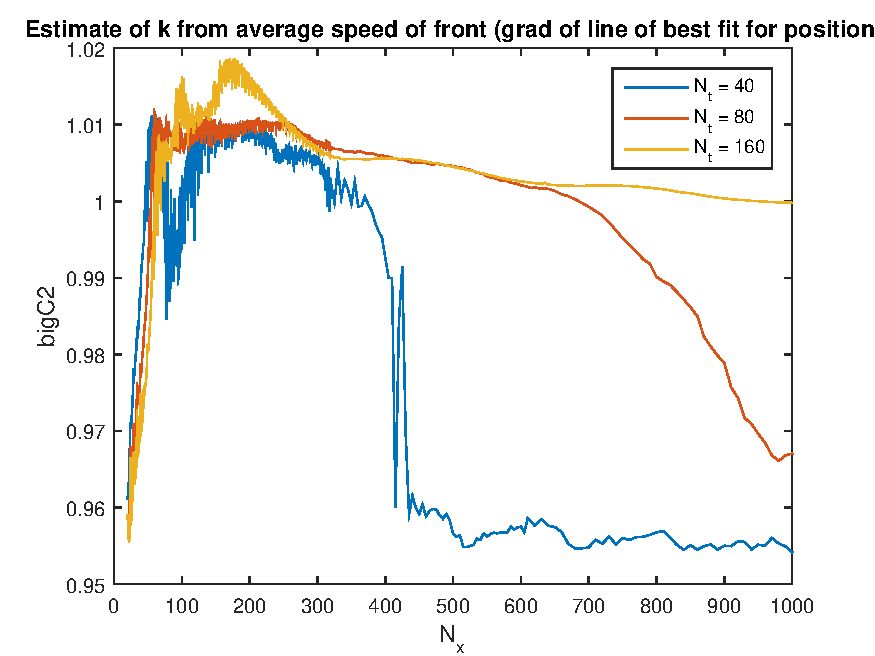
\includegraphics[width=0.9\textwidth]{alan7-k.pdf}
  \caption{Moving mesh as in Figure~\ref{fig:alan4-k}, but with
  $M(u,x) = \sqrt{0.1 + {u_{xx}}^2}$.
  \label{fig:alan7-k}}
\end{figure}

\clearpage
\section{Numerical results for viscosity}

\begin{figure}[htbp]
\centering
  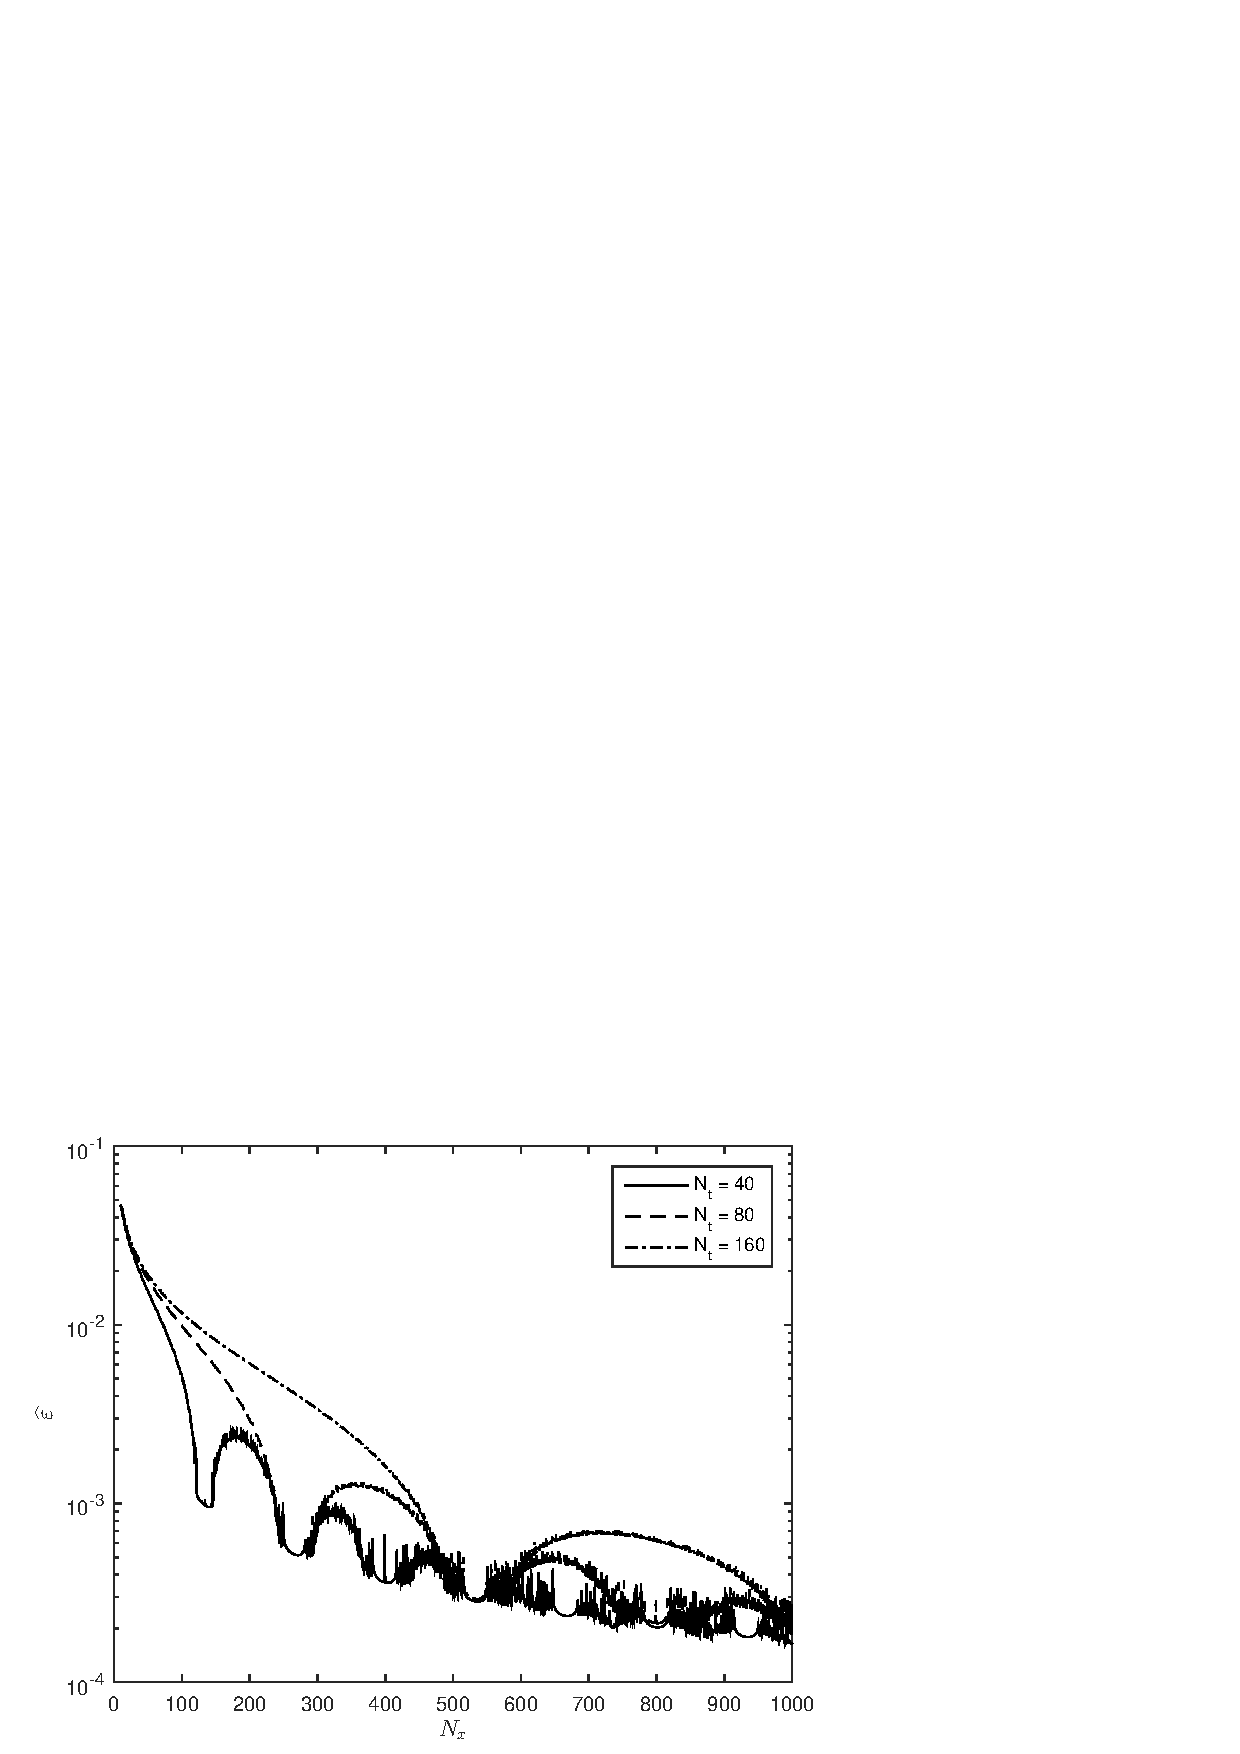
\includegraphics[width=0.9\textwidth]{alan0-eps.pdf}
  \caption{Default parameters: $\alpha = 0.1$, $\theta_u = \theta_x = 0.5$,
  linear interpolation and static mesh.
  \label{fig:alan0-eps}}
\end{figure}
\begin{figure}[hbtp]
\centering
  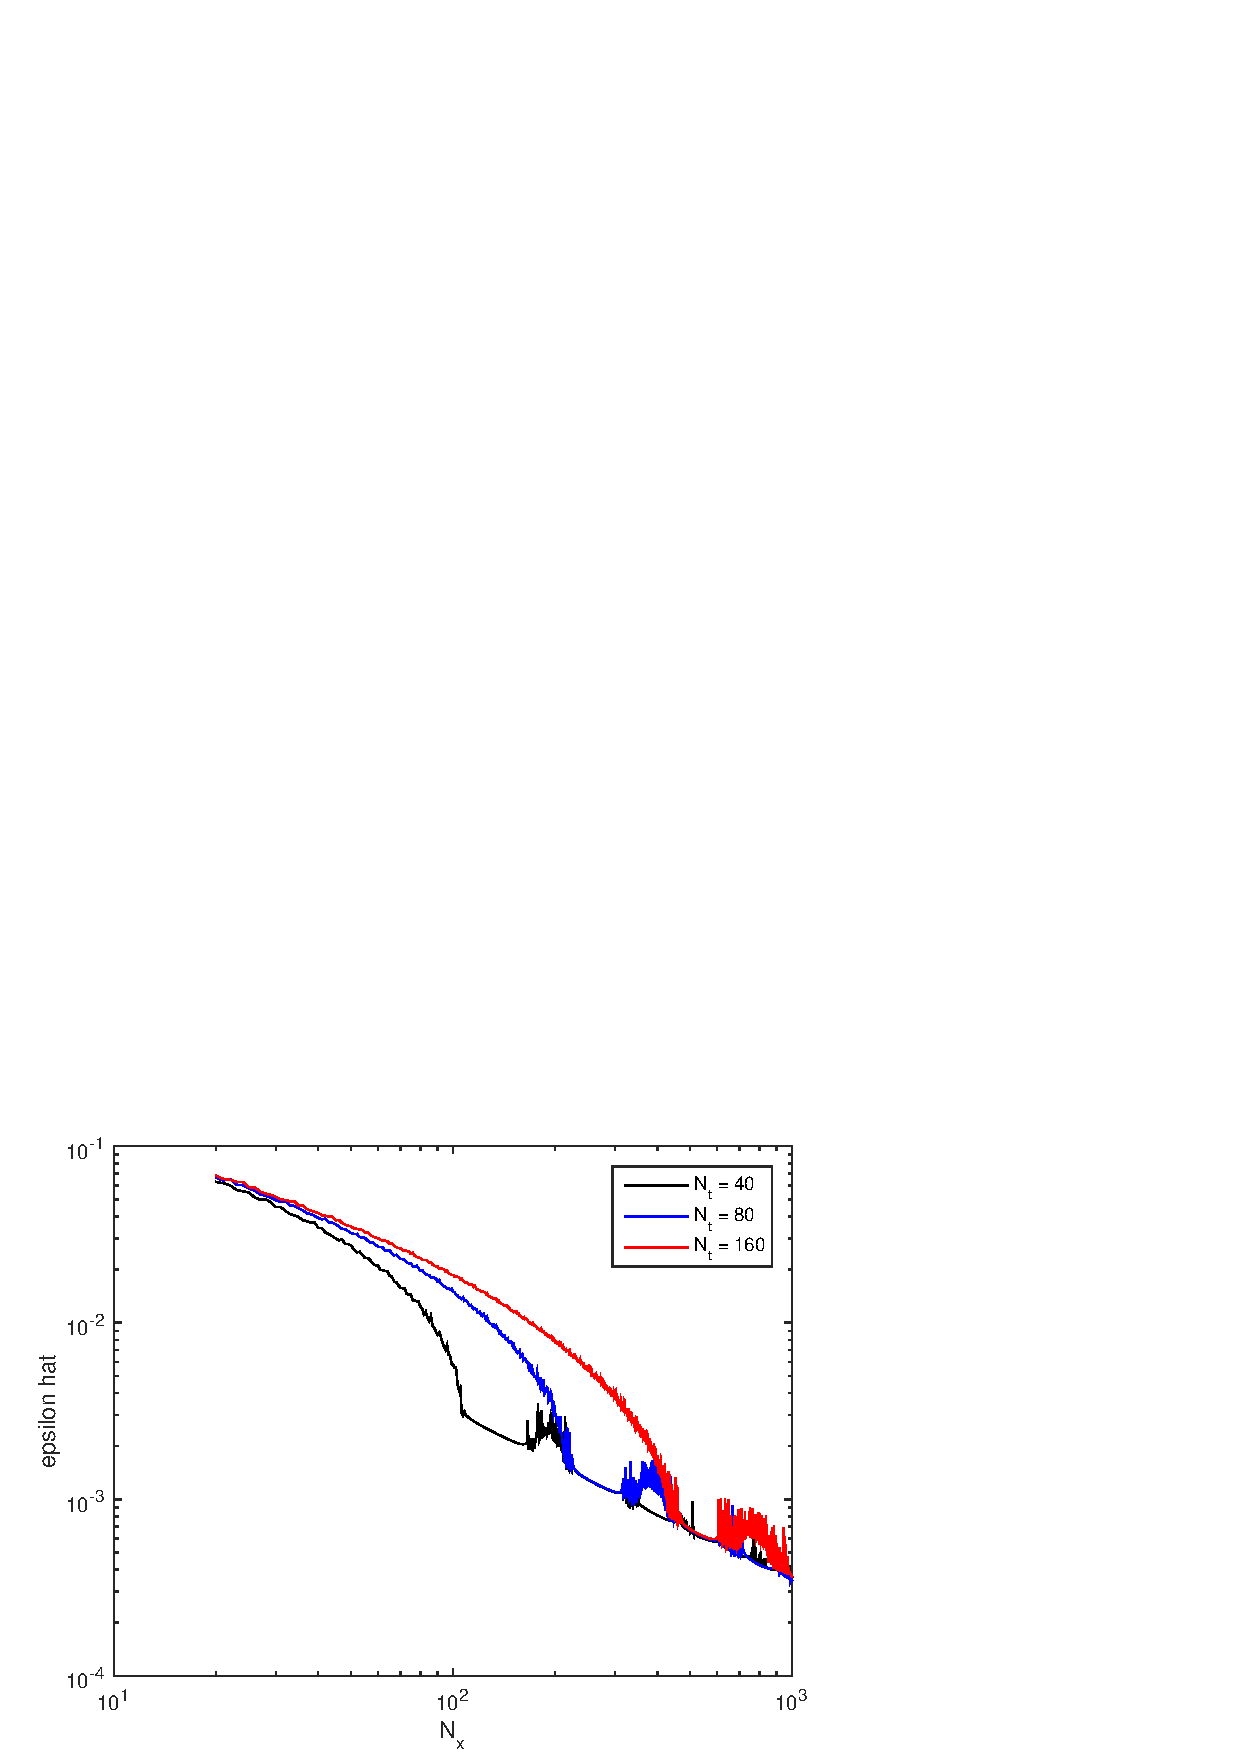
\includegraphics[width=0.9\textwidth]{alan1-eps.pdf}
  \caption{As above, but $\alpha = 0.25$.
  \label{fig:alan1-eps}}
\end{figure}
\begin{figure}[htbp]
\centering
  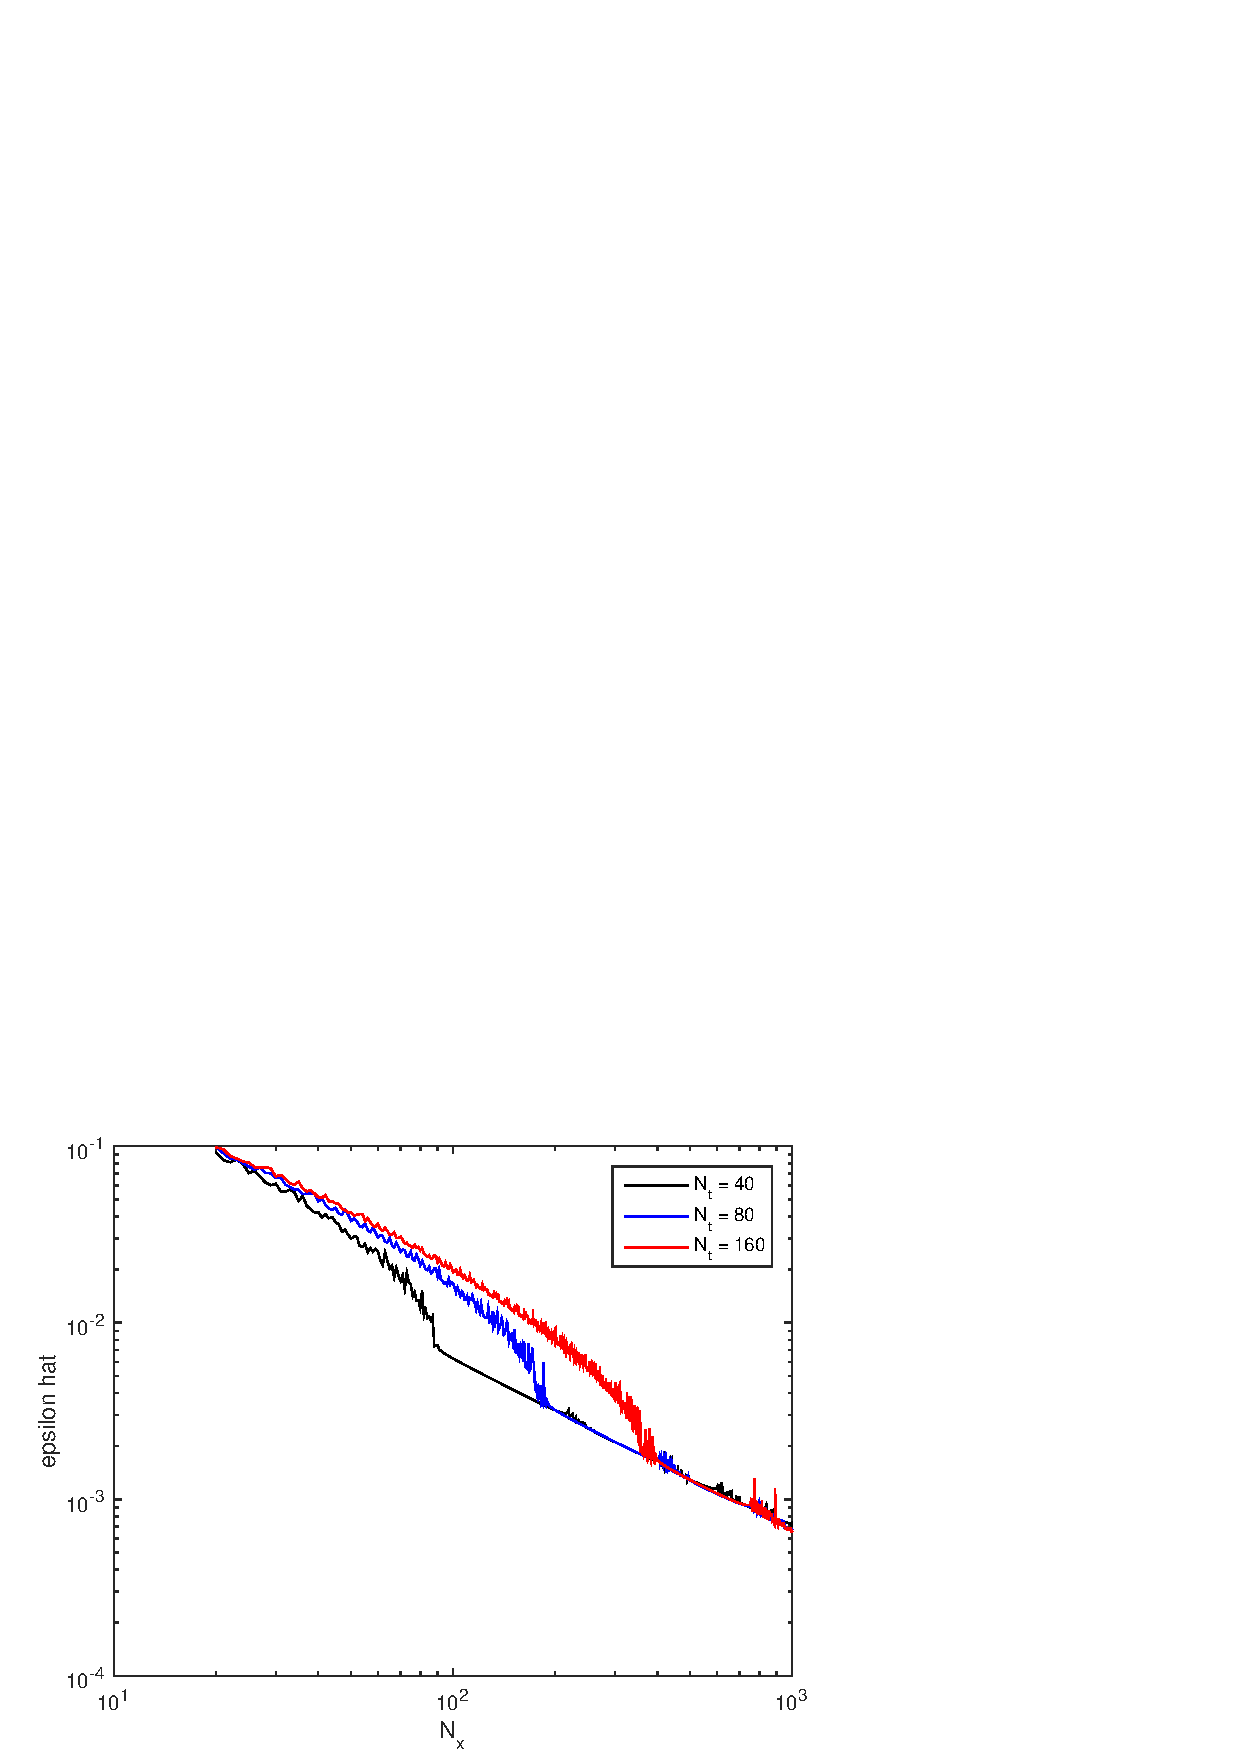
\includegraphics[width=0.9\textwidth]{alan2-eps.pdf}
  \caption{Large wave amplitude, $\alpha = 0.5$.
  \label{fig:alan2-eps}}
\end{figure}
\begin{figure}[hbtp]
\centering
  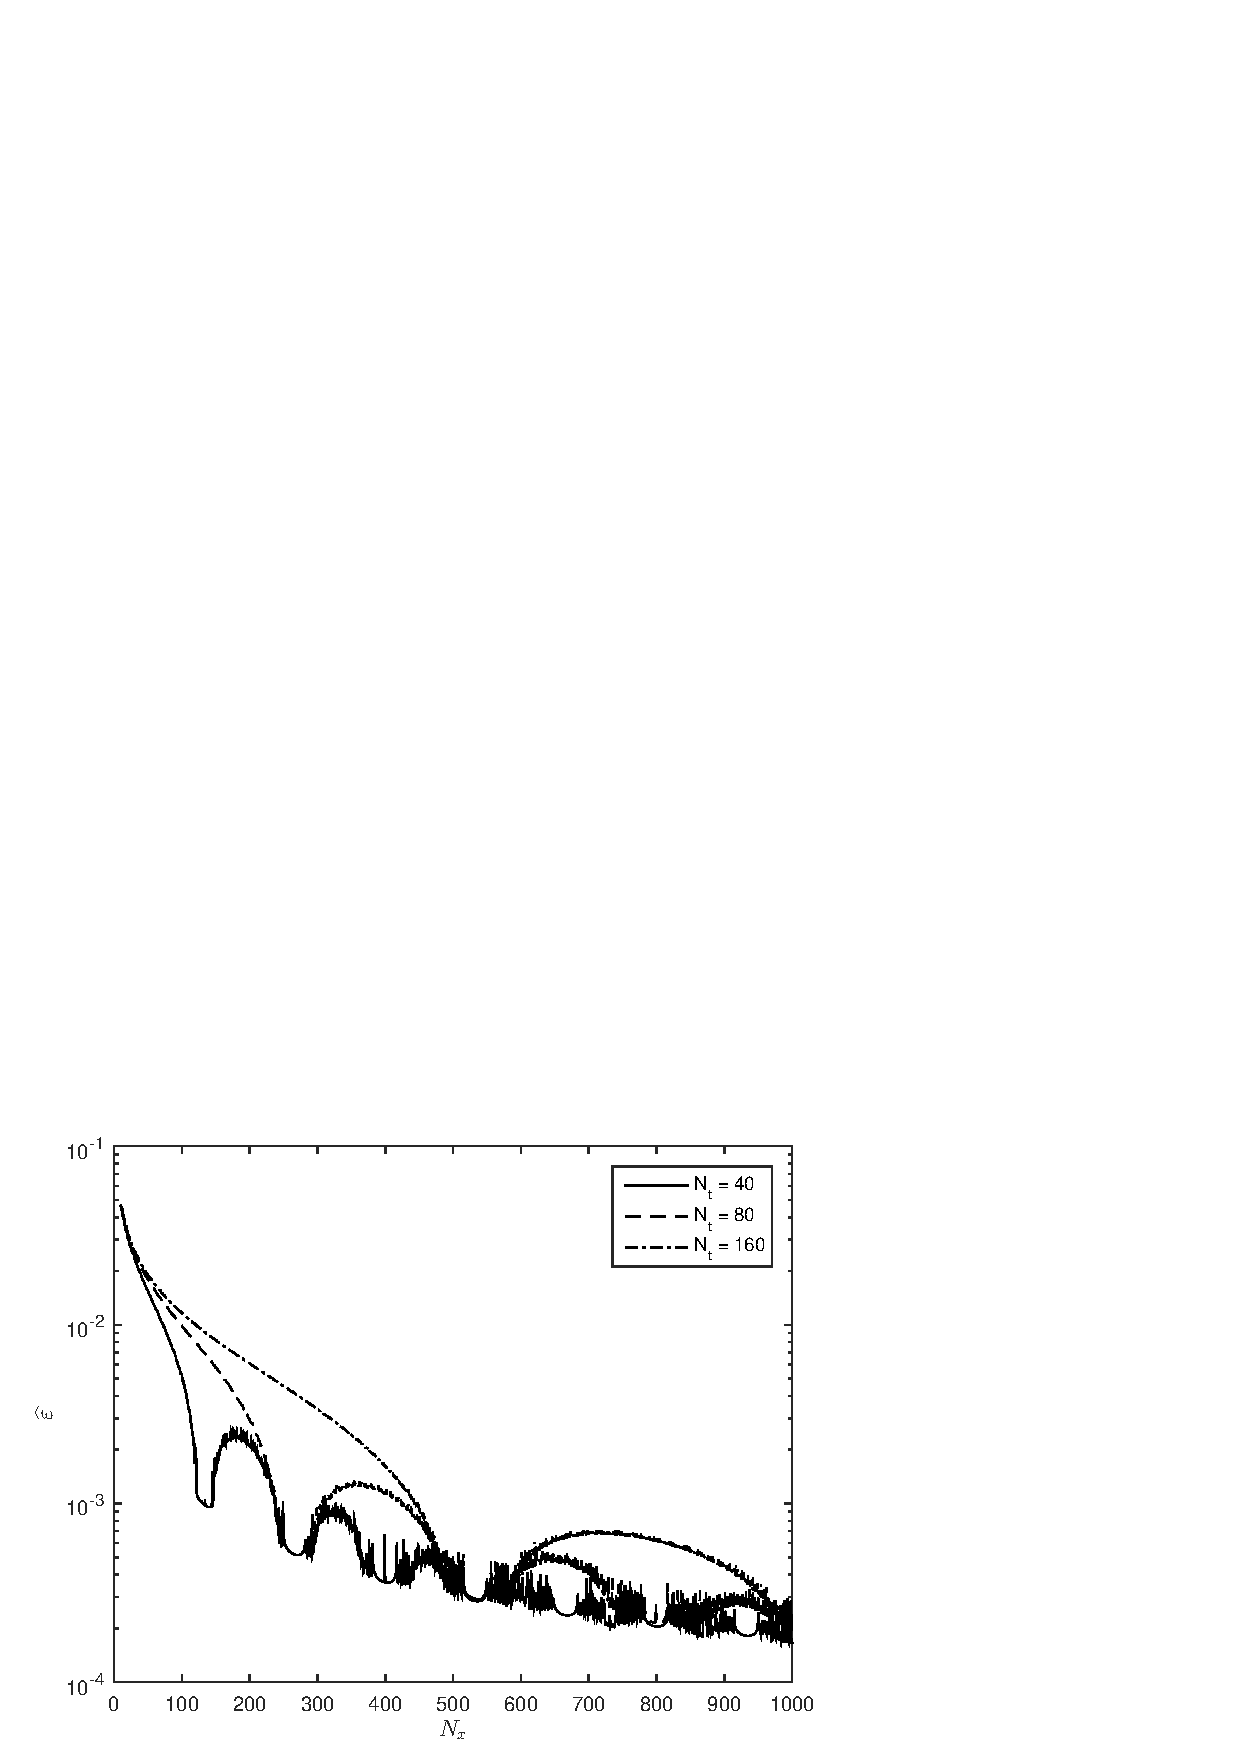
\includegraphics[width=0.9\textwidth]{alan3-eps.pdf}
  \caption{Theta method in place of Crank-Nicholson with $\theta_u = \theta_x = 0.55$.
    Side-by-side, this Figure and Figure~\ref{fig:alan0-eps} are indistinguishable.
  \label{fig:alan3-eps}}
\end{figure}
\begin{figure}[htbp]
\centering
  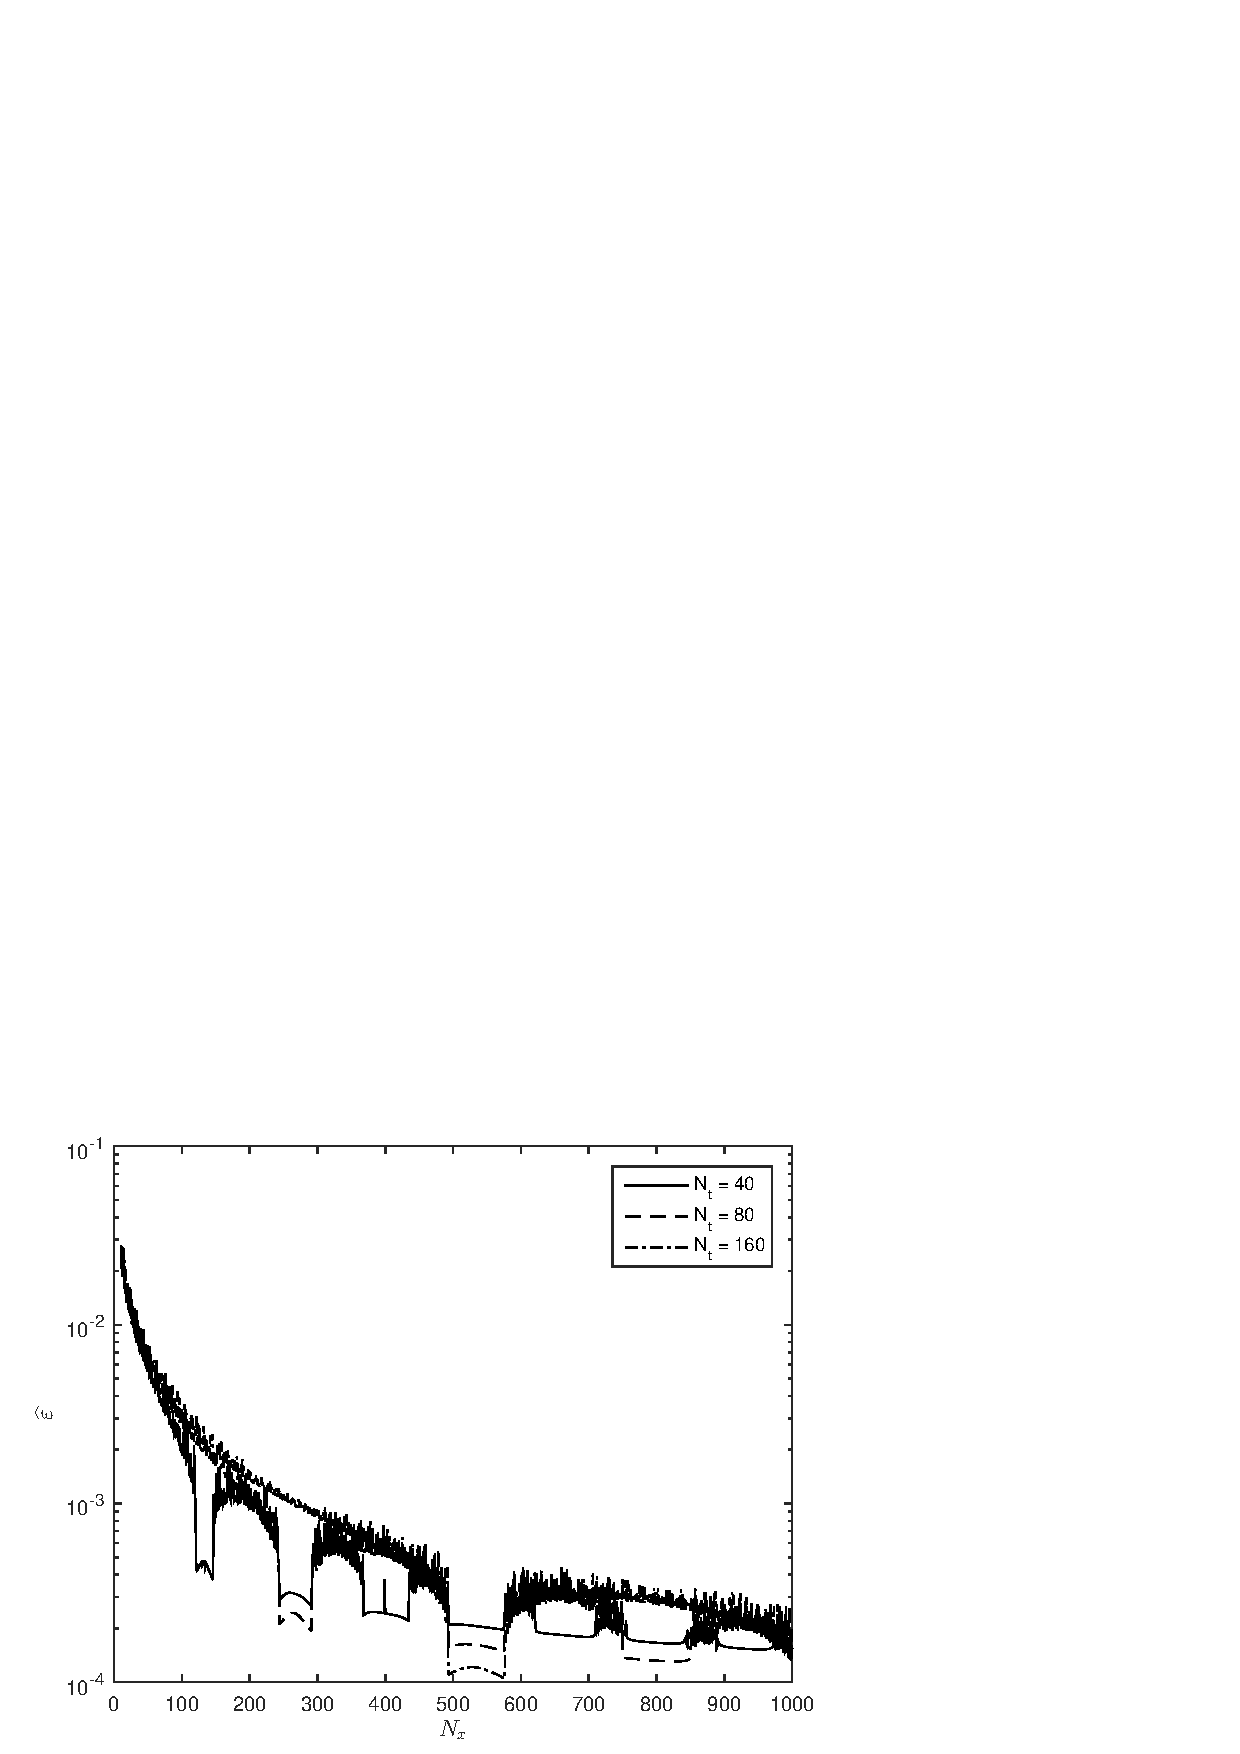
\includegraphics[width=0.9\textwidth]{alan6-eps.pdf}
  \caption{Numerical viscosity with cubic Lagrange interpolation.
  \label{fig:alan6-eps}}
\end{figure}
\begin{figure}[hbtp]
\centering
  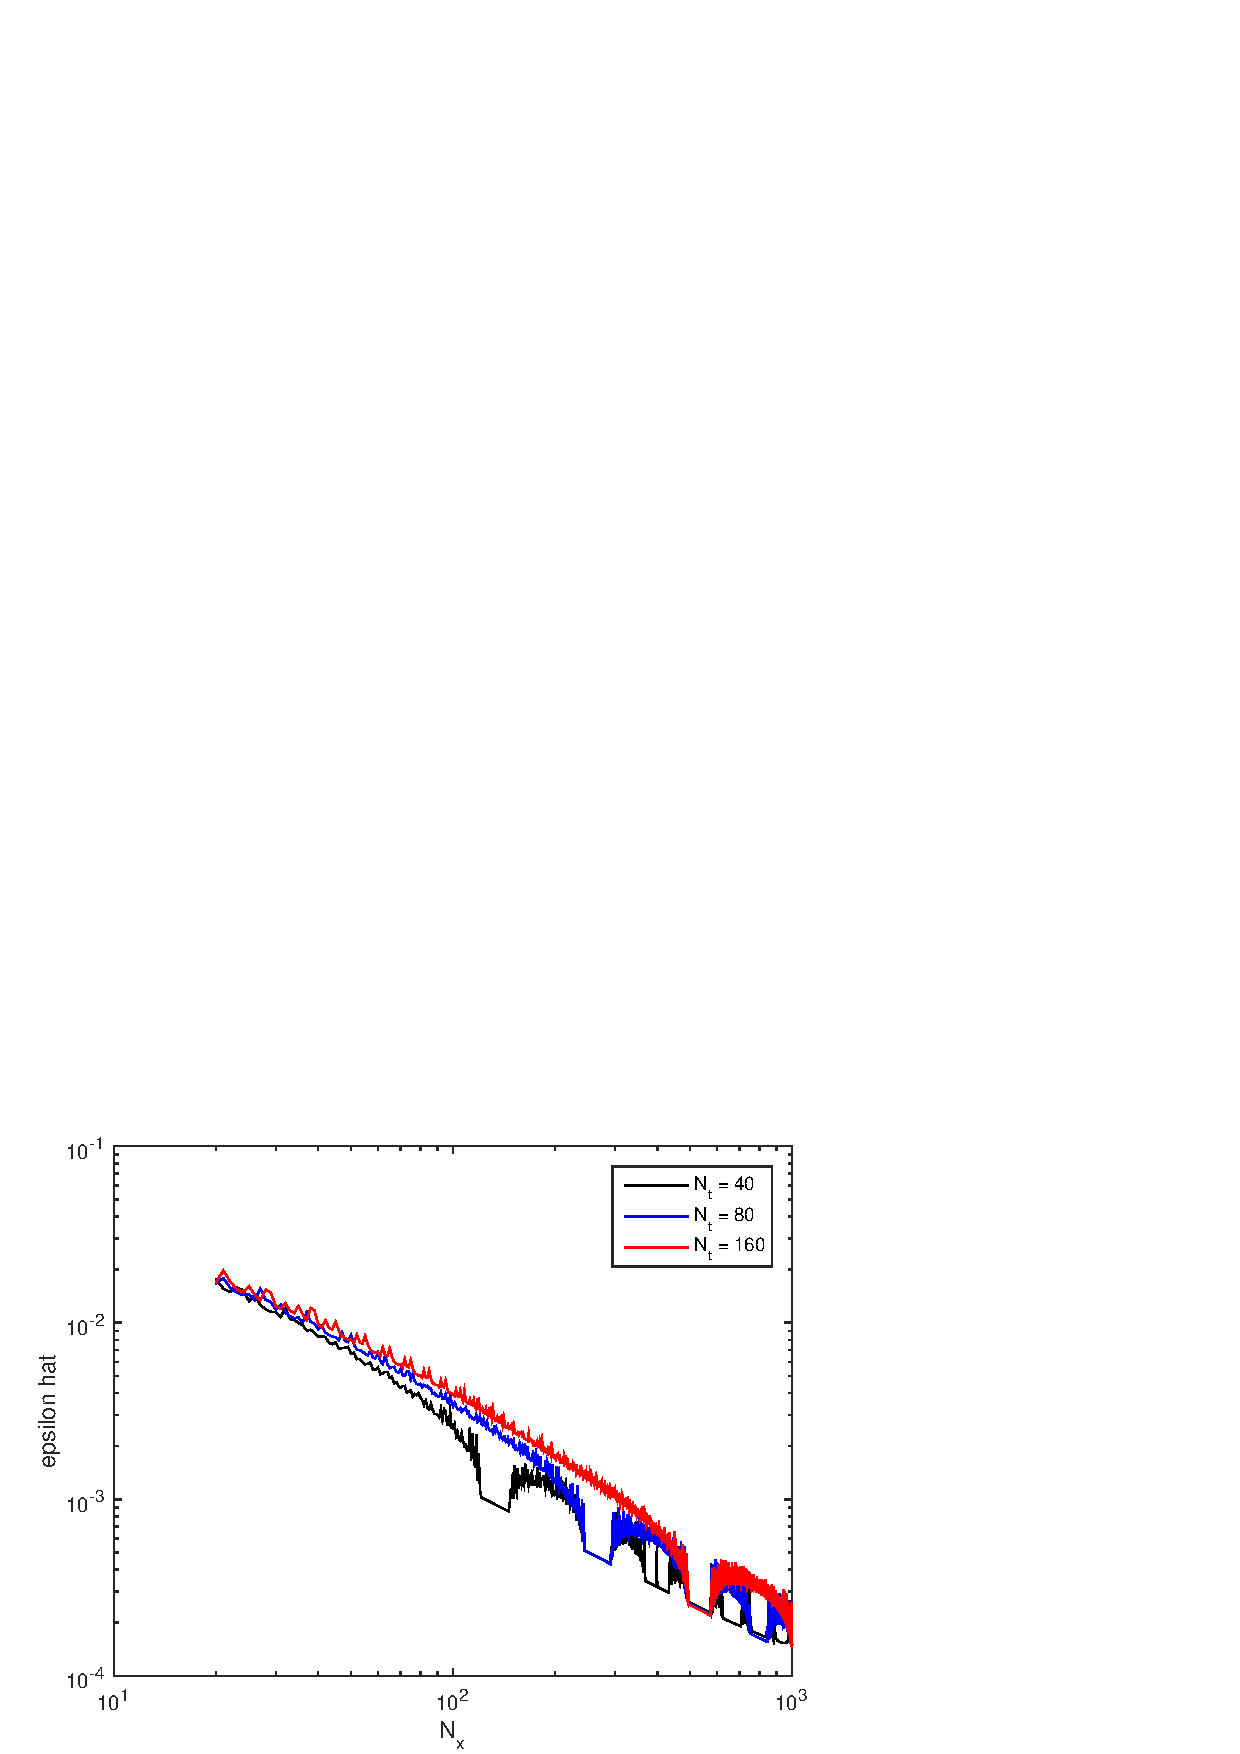
\includegraphics[width=0.9\textwidth]{alan5-eps.pdf}
  \caption{As in Figure~\ref{fig:alan6-eps}, but with an interpolation limiter
  applied, sacrificing smoothness for monotonicity.
  \label{fig:alan5-eps}}
\end{figure}
\begin{figure}[htbp]
\centering
  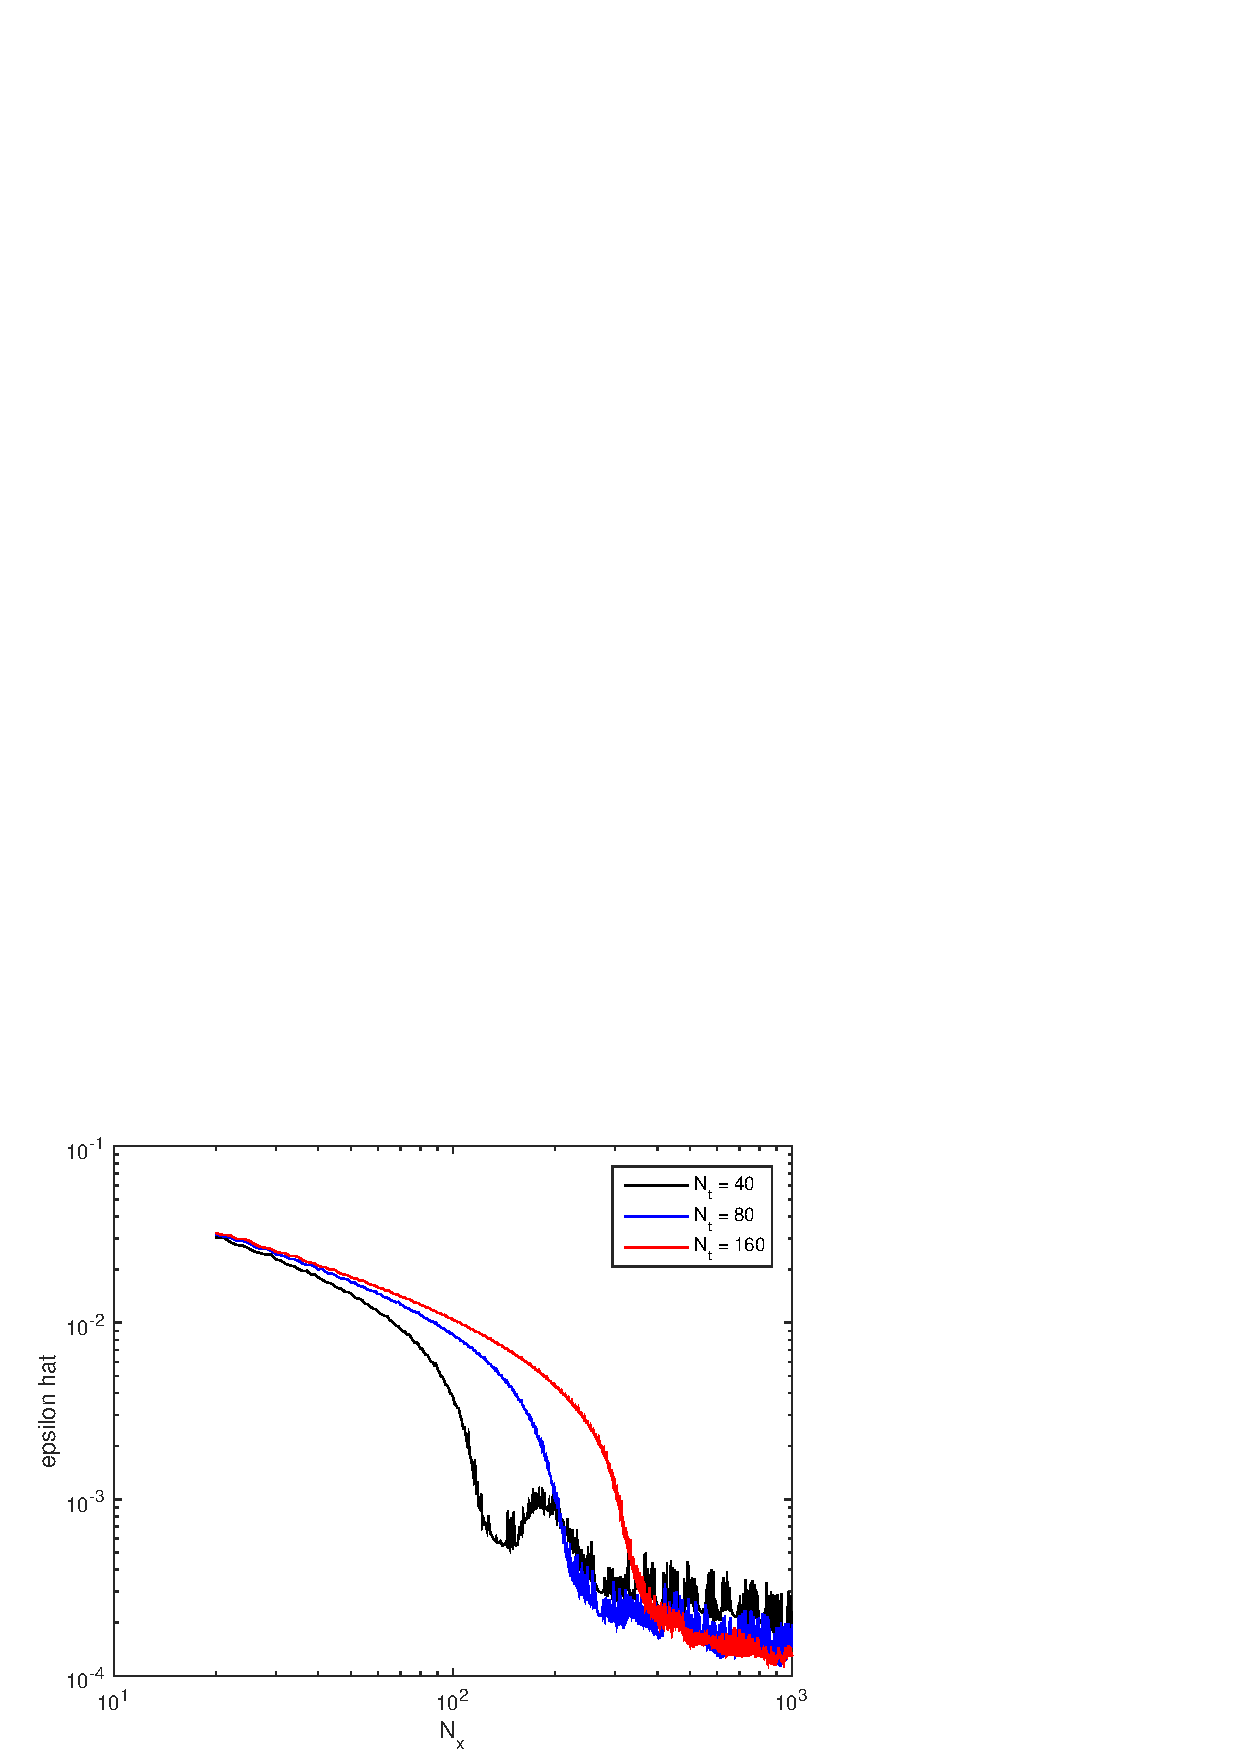
\includegraphics[width=0.9\textwidth]{alan4-eps.pdf}
  \caption{Moving mesh with exact equidistribution, so $X_A^{n+1}$
    equidistributes the linear interpolant of $M(U^n_A,X^n_A)$, with
    $M(u,x) = \sqrt{0.1 + {u_x}^2}$ (after smoothing and normalisation).
  \label{fig:alan4-eps}}
\end{figure}
\begin{figure}[hbtp]
\centering
  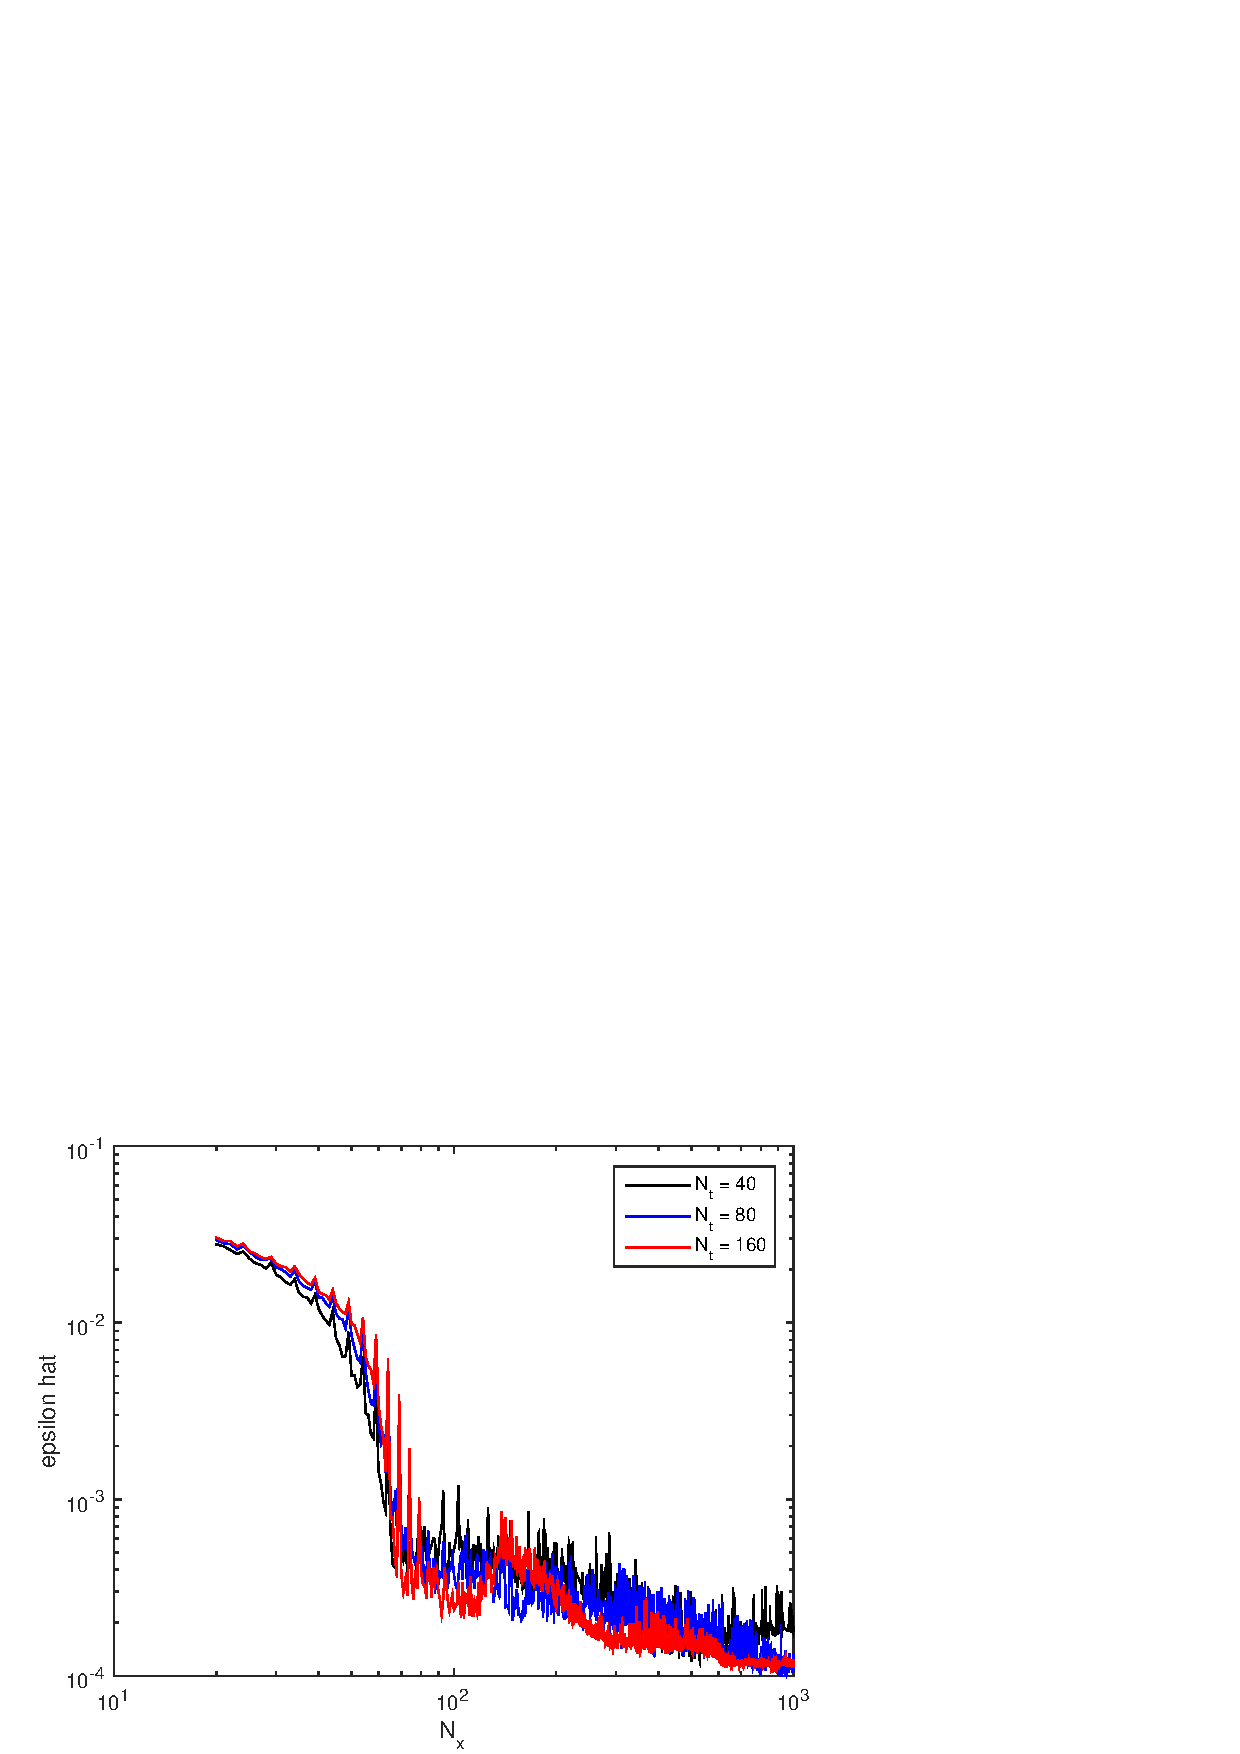
\includegraphics[width=0.9\textwidth]{alan7-eps.pdf}
  \caption{Moving mesh as in Figure~\ref{fig:alan4-eps}, but with
  $M(u,x) = \sqrt{0.1 + {u_{xx}}^2}$.
  \label{fig:alan7-eps}}
\end{figure}

\clearpage
\section{Minimum mesh spacing}

\begin{figure}[hbtp]
\centering
  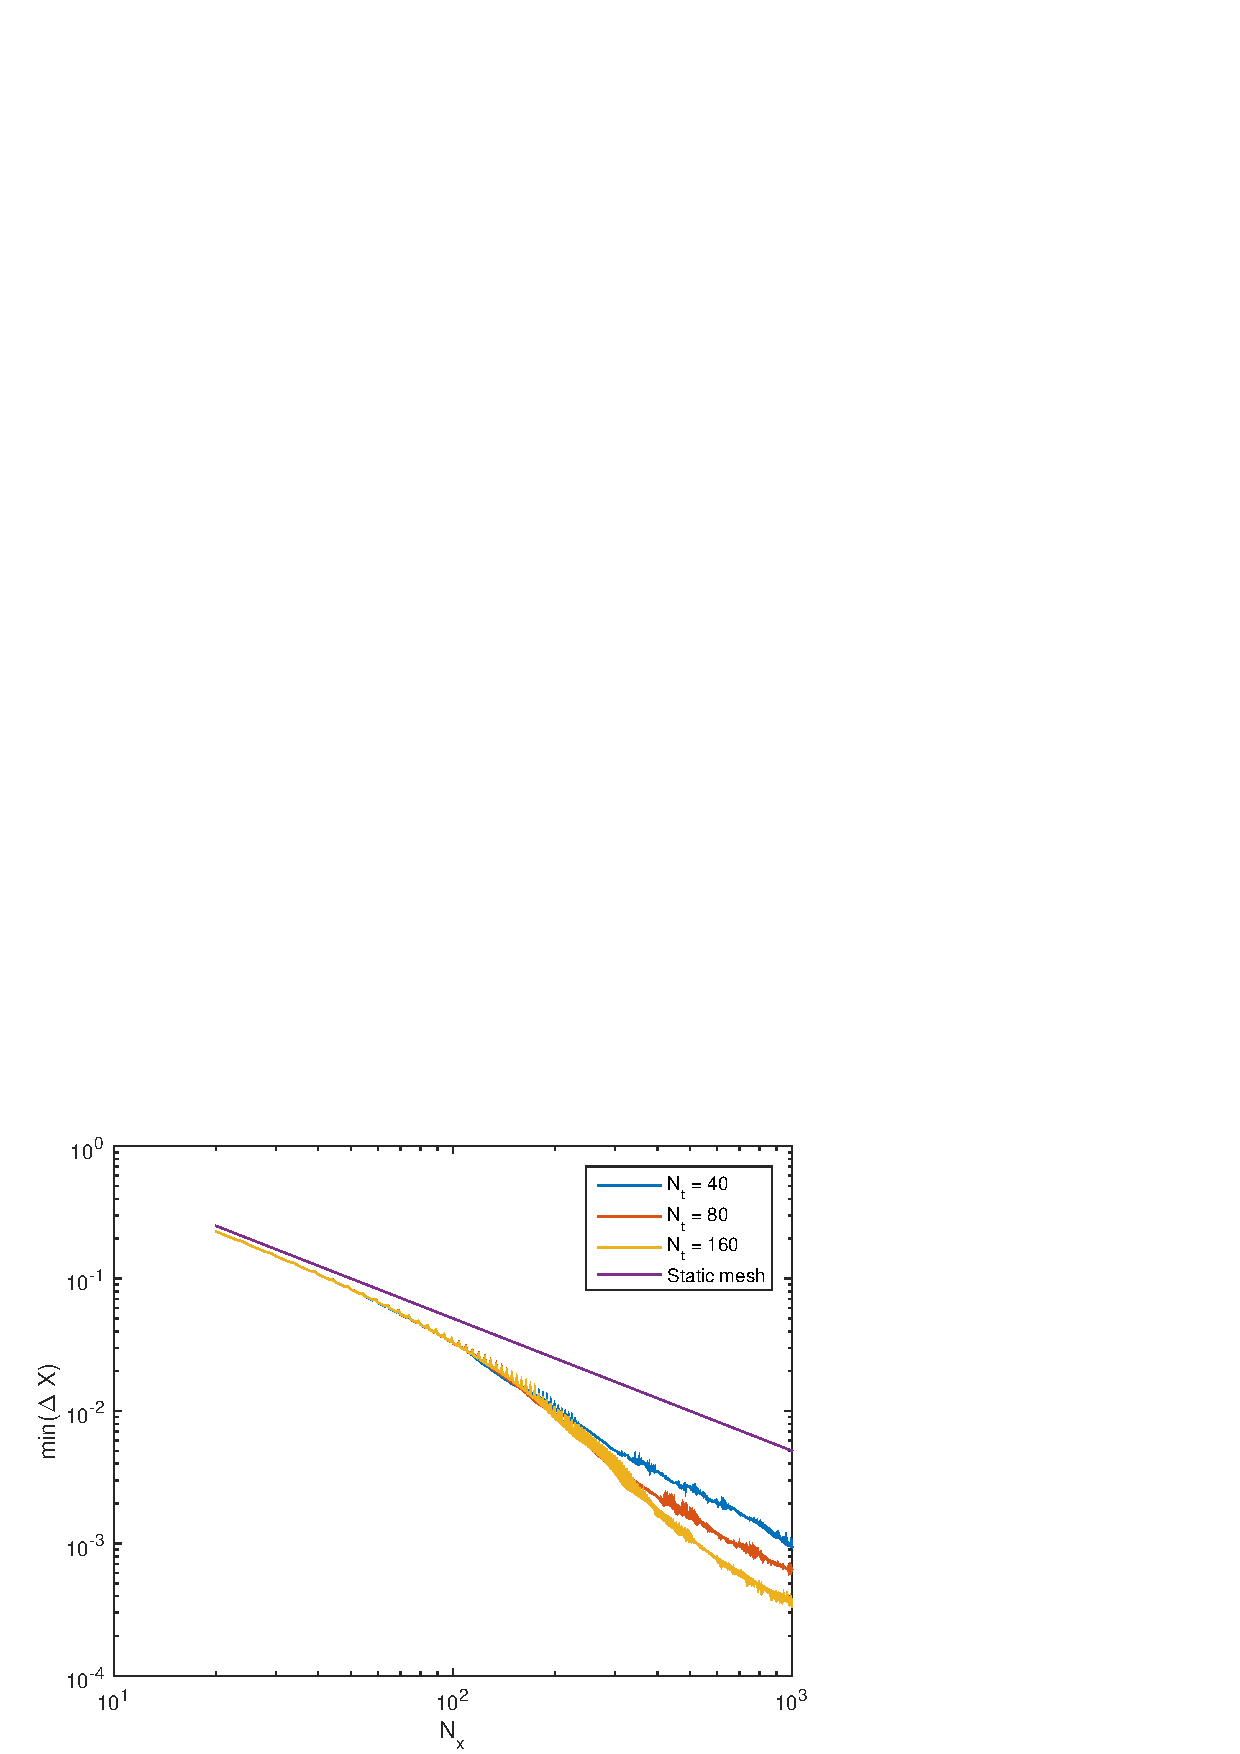
\includegraphics[width=0.9\textwidth]{alan4-minDx.pdf}
  \caption{Minimum mesh spacing for moving mesh with  $M(u,x) = \sqrt{0.1 + {u_{x}}^2}$.
  \label{fig:alan4-minDx}}
\end{figure}
\begin{figure}[hbtp]
\centering
  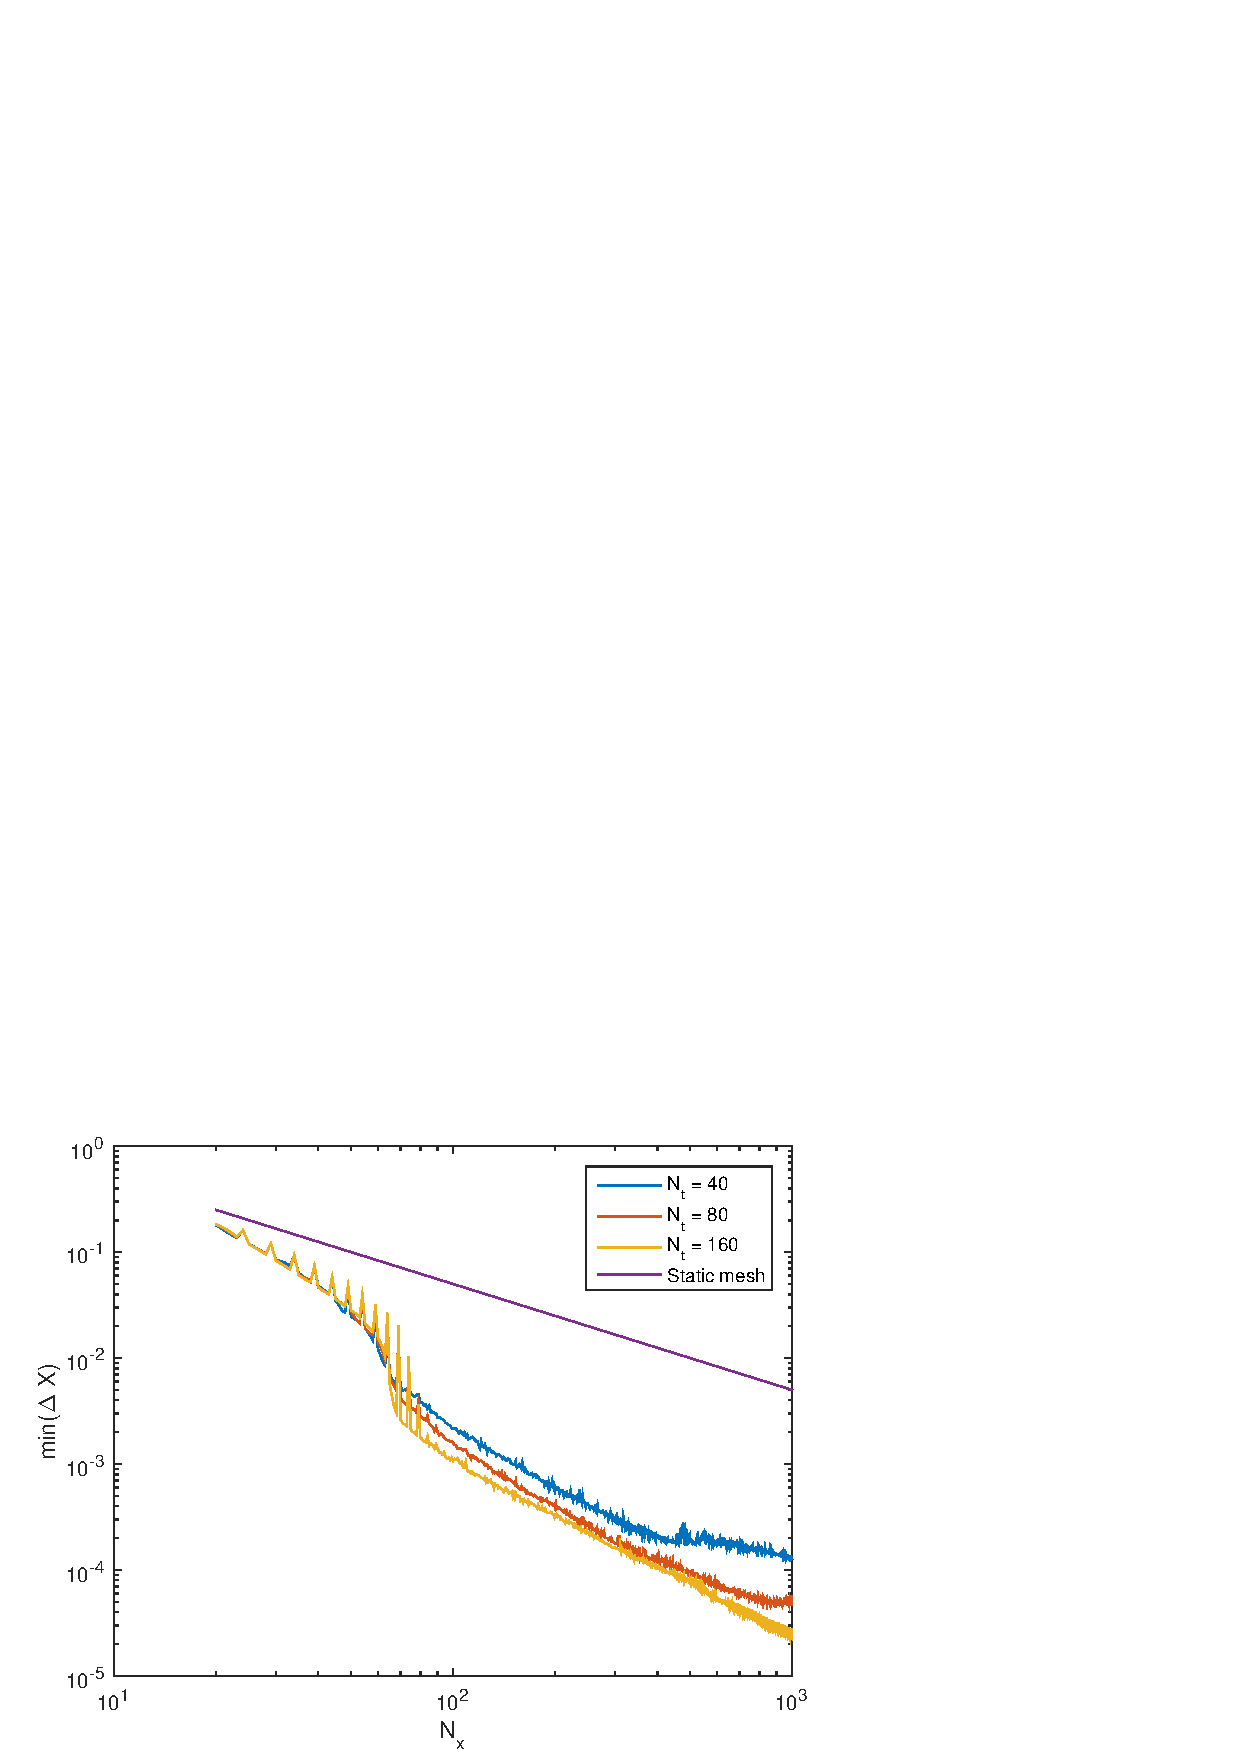
\includegraphics[width=0.9\textwidth]{alan7-minDx.pdf}
  \caption{Minimum mesh spacing for moving mesh with  $M(u,x) = \sqrt{0.1 + {u_{xx}}^2}$.
  \label{fig:alan7-minDx}}
\end{figure}
\begin{figure}[htbp]
\centering
  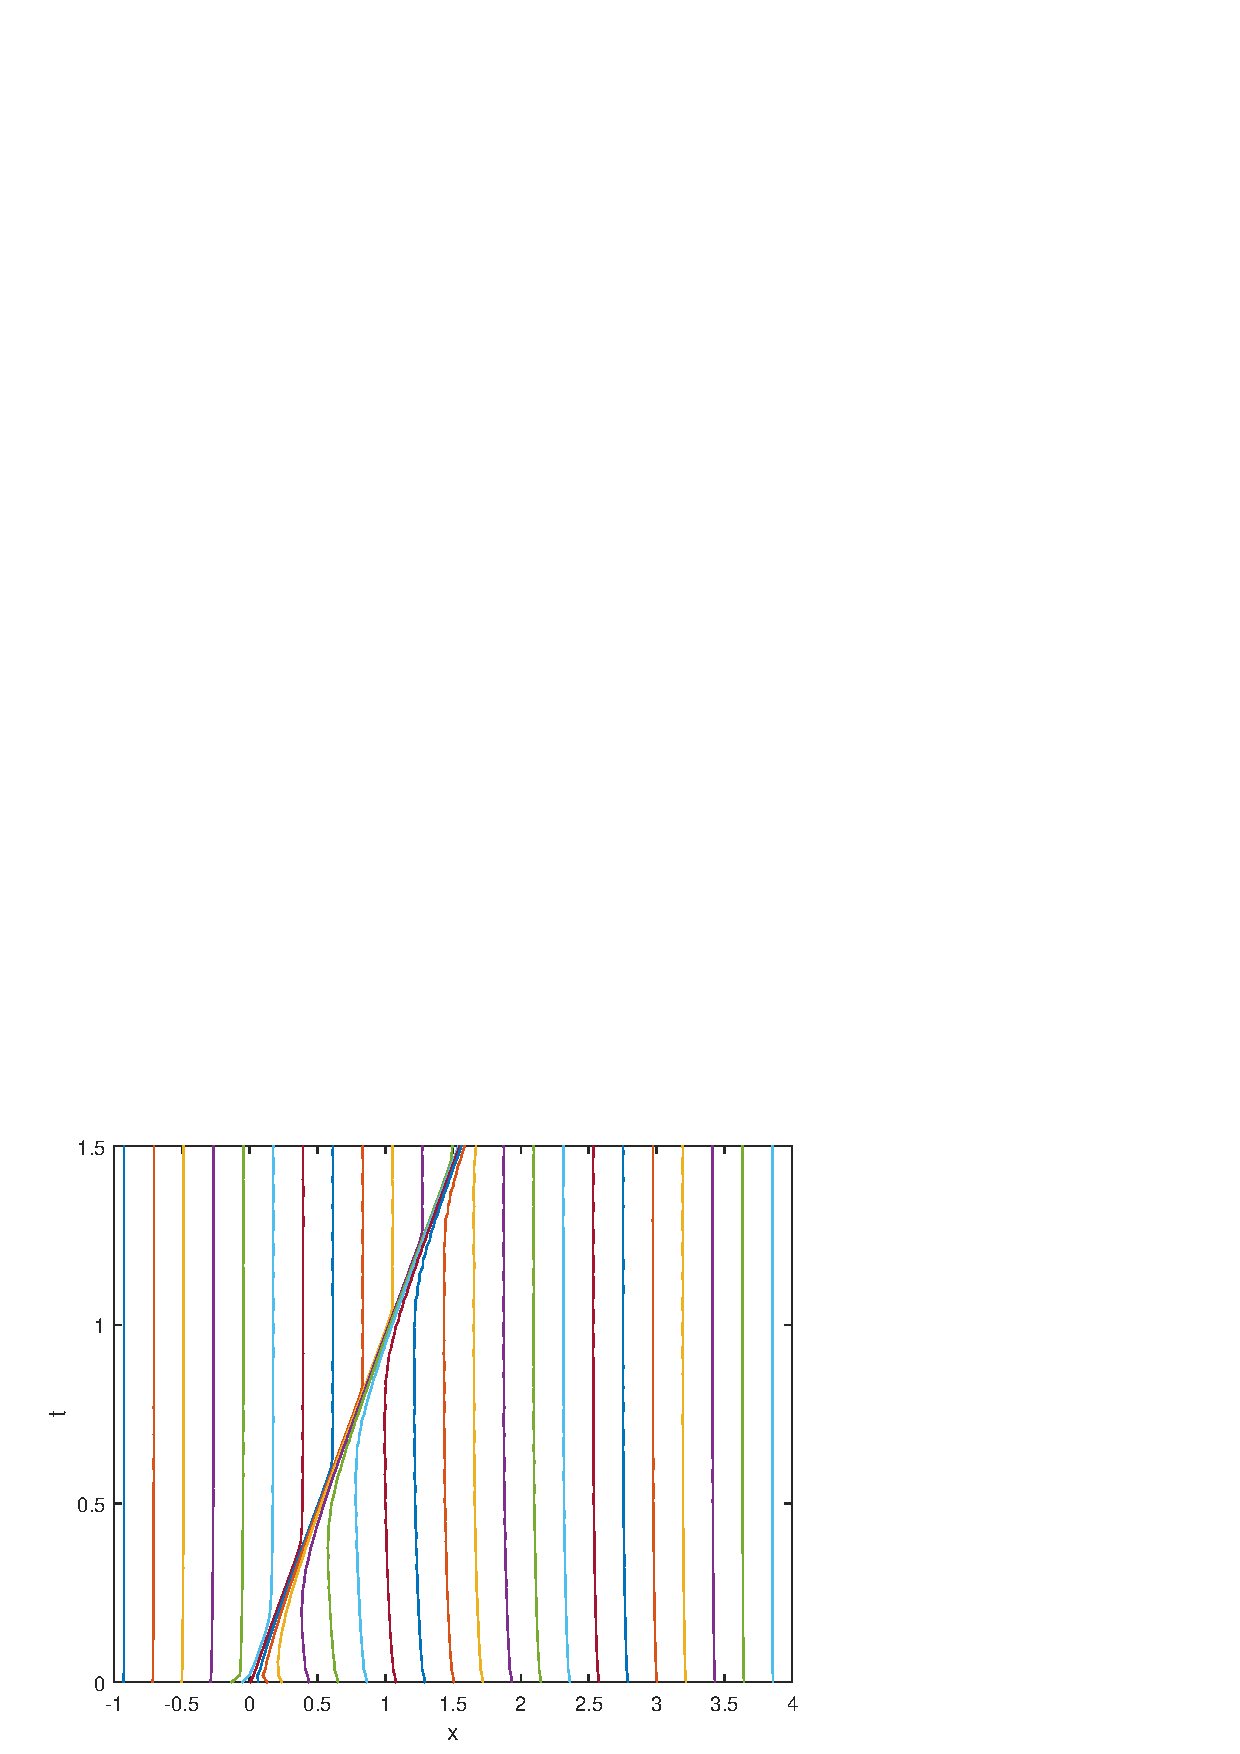
\includegraphics[width=0.9\textwidth]{mm-traj.pdf}
  \caption{Location of the arrival meshpoints over time for $N_x = N_t = 80$ and
  $M(u,x) = \sqrt{0.1 + {u_{xx}}^2}$. Only 26 meshpoints are shown here.
  \label{fig:mm-traj}}
\end{figure}
\begin{figure}[hbtp]
\centering
  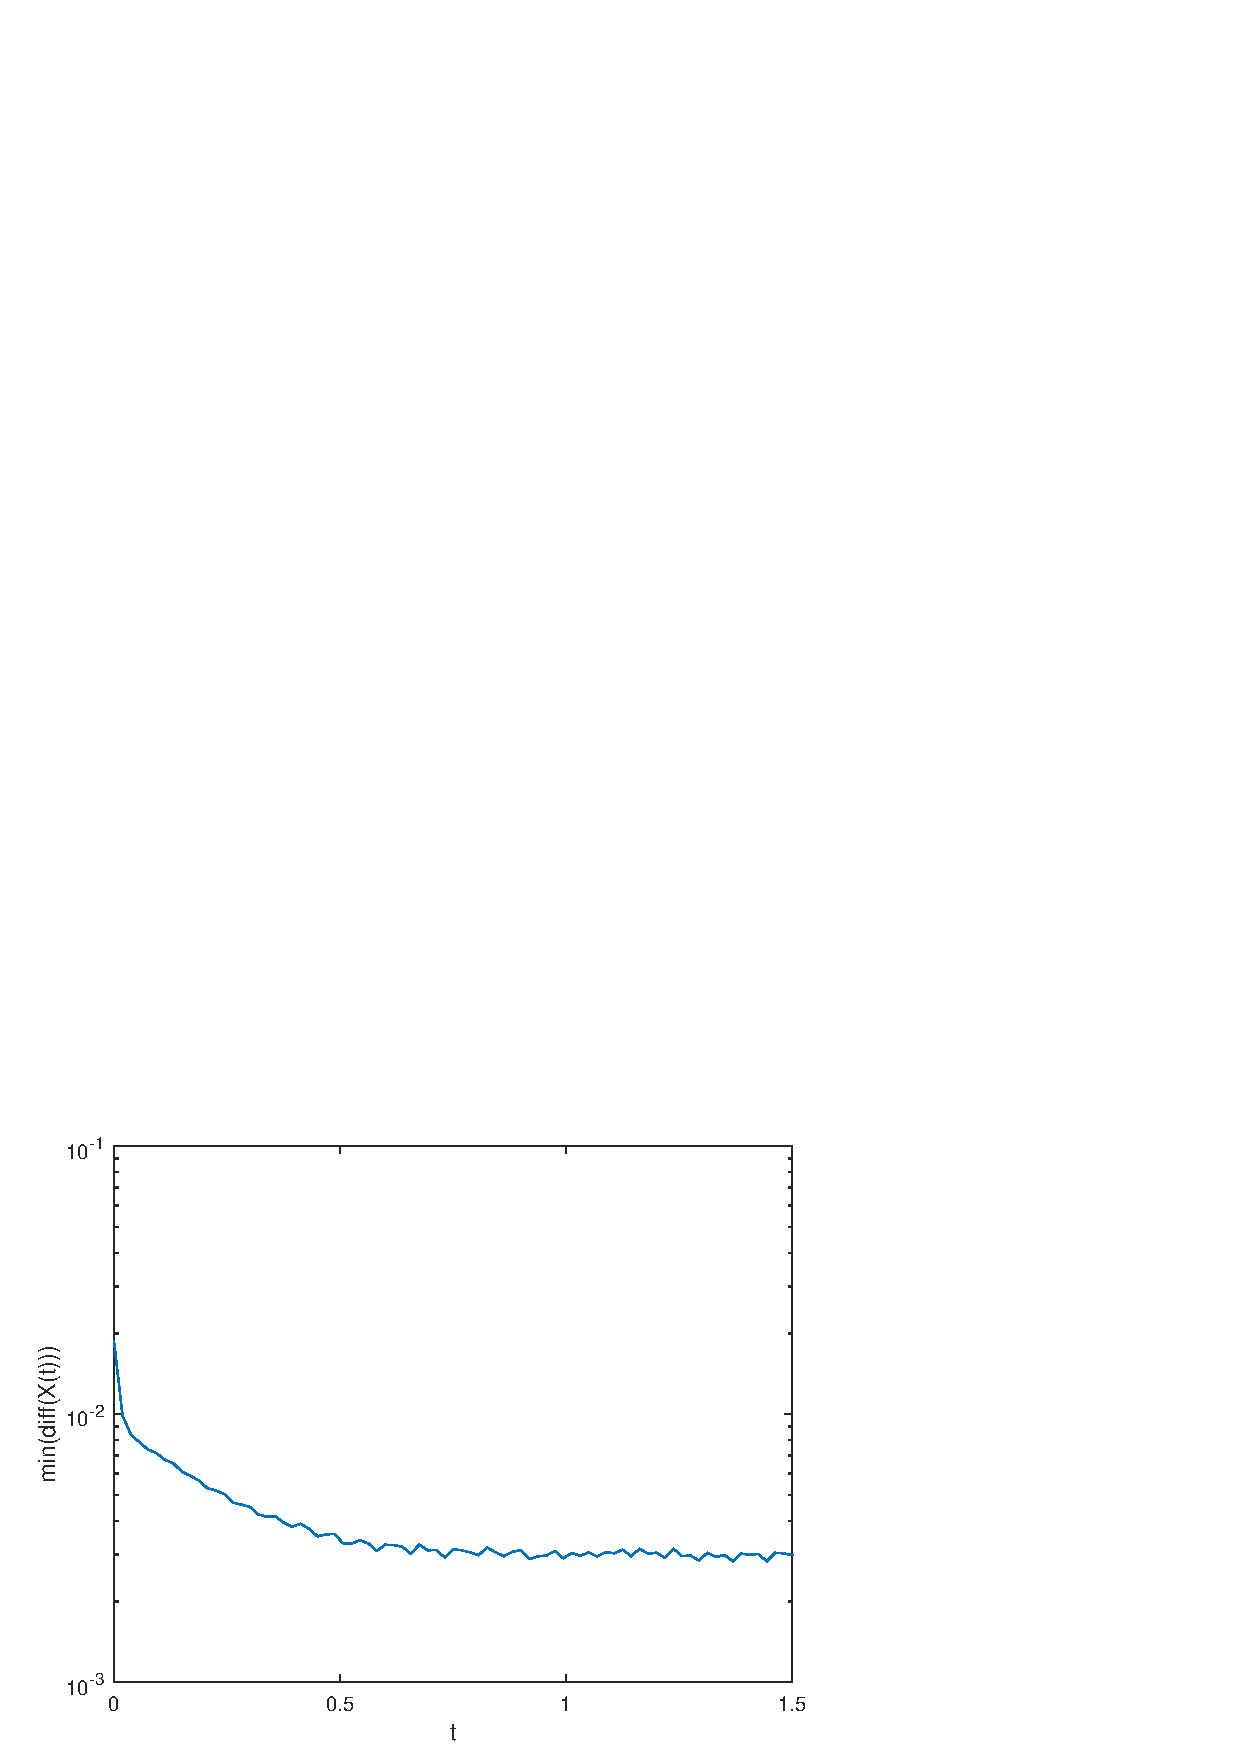
\includegraphics[width=0.9\textwidth]{mm-minDx.pdf}
  \caption{Minimum mesh spacing over time for Figure~\ref{fig:mm-traj}
  \label{fig:mm-minDx}}
\end{figure}

\end{document}
